\documentclass[cn,12pt,chinese]{elegantbook}
\graphicspath{{figures/}{logo/}}

\setCJKfamilyfont{songkeben} {FZSKBXKK.TTF}
\newcommand{\songkeben}{\CJKfamily{songkeben}}
%引用宏包
\usepackage{xcolor}

\begin{document}
\clearpage
\pagecolor[RGB]{248,244,237}
\newcommand{\verticalspace}[1][]{\vspace*{\stretch{#1}}}

\pagestyle{empty}
\begin{center}
    \verticalspace[1.5]
    \Huge {\songkeben 半導體器件物理\\學習筆記}
    
    
    \verticalspace[1]
    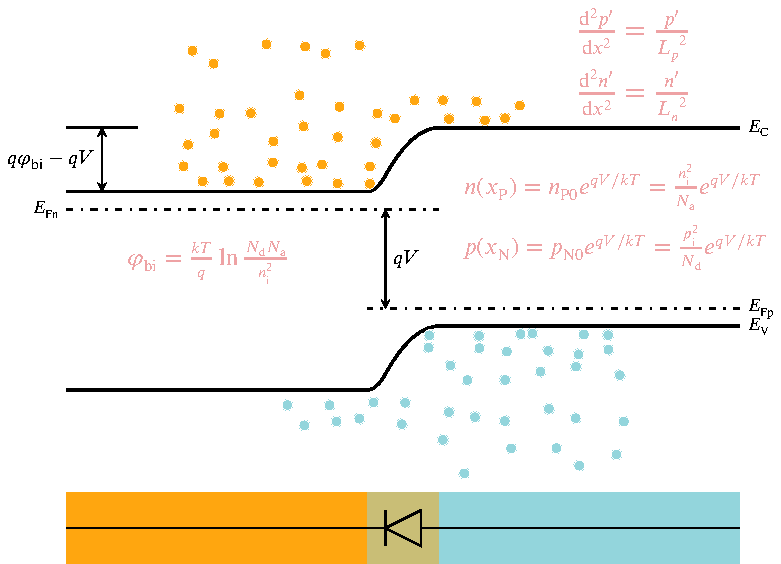
\includegraphics[width = \linewidth]{junction-band.pdf}
\end{center}

\verticalspace[2]
\raggedleft
\Large
{\kaishu 李华康}\\
{\kaishu 中科院电工所}\\
2020.8.21
\clearpage
\pagecolor[rgb]{1, 1, 1}
\chapter{基础知识}


\end{document}

